%!TEX program = xelatex
\documentclass[11pt, a4paper]{article}
  \usepackage[a4paper,top=3cm,bottom=4cm,left=2.5cm,right=2.5cm]{geometry}
  \usepackage{subfig}
  \usepackage{graphicx}
  \graphicspath{{../images/}}
  \usepackage{hyperref}
  \usepackage{amsmath}
  \usepackage{braket}
  \usepackage{enumitem}
  \usepackage{mathtools}
  \usepackage{xepersian}
  \settextfont[Scale=1.2]{B Nazanin}
  \setlatintextfont[Scale=1]{Times New Roman Cyr}
  \title{\textbf{شبیه‌سازی رایانه‌ای در فیزیک}\\تمرین چهارم: ول‌گشت}
  \author{سینا معمر ۹۵۱۰۲۳۱۶}
    

\begin{document}

\maketitle
\thispagestyle{empty}


\section{\textbf{انحراف از معیار}}

\begin{align}
  \braket{x^2(t)} & = \braket{(x(t - \tau) + al)^2} \nonumber \\
           & = \braket{x^2(t - \tau) + 2alx(t - \tau) + a^2 l^2} \nonumber \\
           & = \braket{x^2(t - \tau)} + 2l\braket{a}\braket{x(t - \tau)} + l^2 \braket{a^2} \nonumber \\
           & = \braket{x^2(t - \tau)} + 2l(p - q)\braket{x(t - \tau)} + l^2 (p + q) \nonumber \\
           & = \braket{x^2(t - \tau)} + 2l(p - q) \Big(\frac{l}{\tau}(p - q)(t - \tau)\Big) + l^2 (p + q) \nonumber \\
           & = \braket{x^2(t - \tau)} + \frac{2l^2}{\tau}(p - q)^2 (t - \tau) + l^2 (p + q) \nonumber \\
           & = \braket{x^2(t - \tau)} + \frac{2l^2}{\tau} (p - q)^2 t - 2l^2 (p - q)^2 + l^2 (p + q) \nonumber \\
           & = l^2 \frac{t}{\tau} \Big((p - q)^2 (\frac{t}{\tau} + 1) - 2(p - q)^2 + (p + q)\Big)
  \label{ean:q1_x_2}
\end{align}

\begin{align}
  \sigma^2(t) & = \braket{x^2(t)} - \braket{x(t)}^2 \nonumber \\
  \xRightarrow{\eqref{ean:q1_x_2}}
           & = l^2 \frac{t}{\tau} \Big((p - q)^2 (\frac{t}{\tau} + 1) - 2(p - q)^2 + (p + q) - (p - q)^2 \frac{t}{\tau} \Big) \nonumber \\
           & = l^2 \frac{t}{\tau} \Big((p - q)^2 - 2(p - q)^2 + (p + q)\Big) \nonumber \\
           & = l^2 \frac{t}{\tau} \Big((p + q) - (p - q)^2\Big) \nonumber \\
           & = l^2 \frac{t}{\tau} \Big(p - p^2 + q - q^2 + 2pq\Big) \nonumber \\
           & = l^2 \frac{t}{\tau} \Big(p(1 - p) + q(1 - q) + 2pq\Big) \nonumber \\
           & = l^2 \frac{t}{\tau} \Big(pq + qp + 2pq\Big) \nonumber \\
           & = \frac{4l^2}{\tau} pqt
\end{align}


\section{\textbf{ول‌گشت}}
کد این قسمت از تمرین در فایل
\lr{q2.py}
قابل مشاهده است.
در ابتدا باید یک
\lr{object}
از کلاس
\lr{RandomWalk}
بسازیم.
سپس تابع
\lr{render}
را با زمان و احتمال دل‌خواه فراخوانی می‌کنیم.
روش کار این تابع به این صورت است که به اندازه‌ی زمان داده شده،
به طور رندوم از بین دو عدد
$1$
و
$-1$
با احتمال داده‌شده انتخاب می‌کند و آن‌ها را در متغیر
\lr{self.steps}
ذخیره می‌کند.
سپس برای به دست آوردن مکان نهایی در زمان‌های مورد نظر، تابع
\lr{calc\_positions}
را صدا می‌زنیم.
این تابع قدم‌ها را به صورت تجمیعی جمع می‌کند و در خانه‌ی متناظر با آن زمان ذخیره می‌کند.
برای این که به طور آماری میانگین آن را به دست بیاوریم،
باید تابع
\lr{calc\_mean\_positions}
را با زمان، طول گام‌ها، احتمال‌ها و تعداد نمونه‌های مورد نظر فراخوانی کنیم.
سپس داده‌های به دست آمده را در متغیر
\lr{sample\_positions\_ensemble}
ذخیره کرده و آن را برای استفاده‌های بعدی در فایلی با فرمت
\lr{.npy}
می‌نویسیم.
واریانس و میانگین داده‌های به دست آمده را برای احتمال‌های
$0.2$،
$0.5$
و
$0.8$
در شکل‌های
\ref{fig:q2_0.2_x}
تا
\ref{fig:q2_0.8_var}
می‌توان مشاهده نمود.
شیب خط فیت شده به هر یک از این نمودار‌ها در جدول
\ref{tab:q2_slopes}
ذکر شده است.

\begin{table}[h!]
  \centering
  \begin{tabular}{|c|c|c|c|}
    \hline
    $0.8$ & $0.5$ & $0.2$ & $p$ \\ \hline
    $0.600$ & $0.000$ & $-0.600$ & $\frac{l}{\tau} (p - q)$ \\ \hline
    $0.642$ & $1.001$ & $0.640$ & $\frac{4l^2}{\tau} pq$ \\ \hline
  \end{tabular}
  \caption{شیب خطوط فیت شده به نمودار‌های میانگین و واریانس مکان ول‌گشت}
  \label{tab:q2_slopes}
\end{table}

همان‌طور که دیده می‌شود نتایج به دست آمده، مطابق با پیش‌بینی ما از تئوری هستند.

\begin{figure}[h!]
	\centering
  \begin{minipage}[b]{0.48\textwidth}
    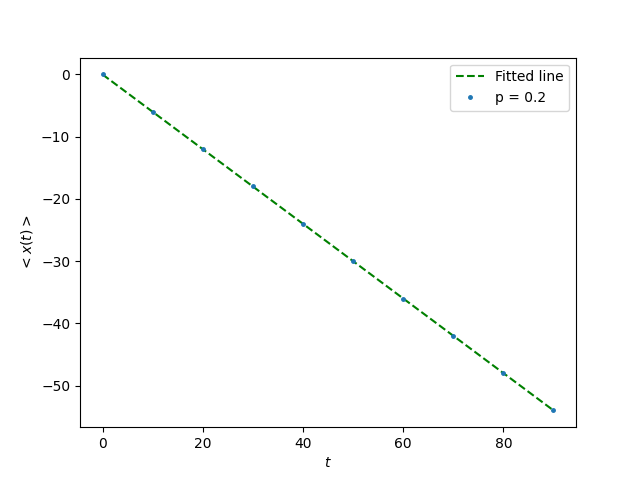
\includegraphics[width=\textwidth]{q2_x_0.2_100_10_100000.png}
    \caption{تغییرات میانگین مکان بر حسب زمان برای $p = 0.2$، $l = 1$، $\tau = 1$ و با $100\,000$ بار تکرار}
    \label{fig:q2_0.2_x}
  \end{minipage}
  \hfill
  \begin{minipage}[b]{0.48\textwidth}
    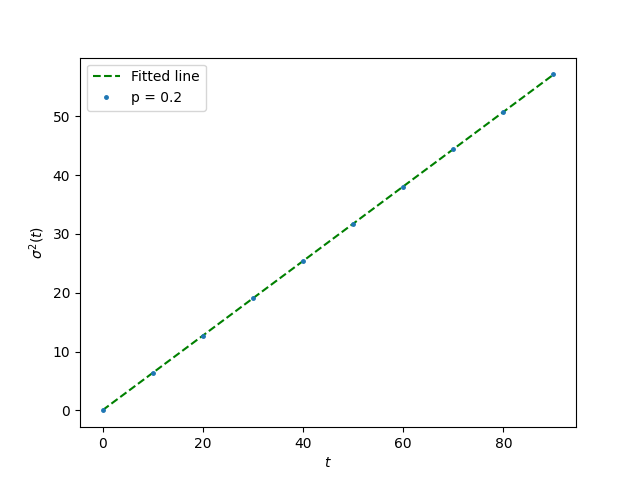
\includegraphics[width=\textwidth]{q2_var_0.2_100_10_100000.png}
    \caption{تغییرات واریانس مکان بر حسب زمان برای $p = 0.2$، $l = 1$، $\tau = 1$ و با $100\,000$ بار تکرار}
    \label{fig:q2_0.2_var}
  \end{minipage}
  \centering
  \begin{minipage}[b]{0.48\textwidth}
    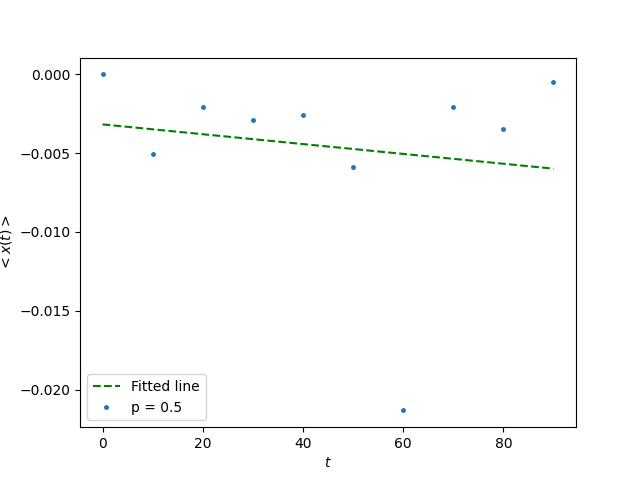
\includegraphics[width=\textwidth]{q2_x_0.5_100_10_100000.png}
    \caption{تغییرات میانگین مکان بر حسب زمان برای $p = 0.5$، $l = 1$، $\tau = 1$ و با $100\,000$ بار تکرار}
    \label{fig:q2_0.5_x}
  \end{minipage}
  \hfill
  \begin{minipage}[b]{0.48\textwidth}
    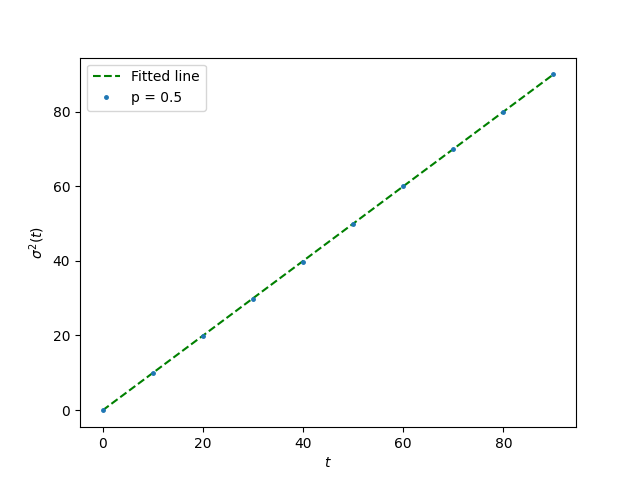
\includegraphics[width=\textwidth]{q2_var_0.5_100_10_100000.png}
    \caption{تغییرات واریانس مکان بر حسب زمان برای $p = 0.5$، $l = 1$، $\tau = 1$ و با $100\,000$ بار تکرار}
    \label{fig:q2_0.5_var}
  \end{minipage}
  \centering
  \begin{minipage}[b]{0.48\textwidth}
    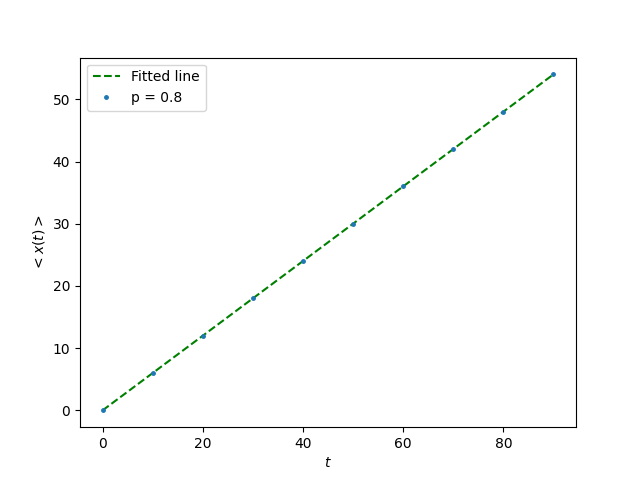
\includegraphics[width=\textwidth]{q2_x_0.8_100_10_100000.png}
    \caption{تغییرات میانگین مکان بر حسب زمان برای $p = 0.8$، $l = 1$، $\tau = 1$ و با $100\,000$ بار تکرار}
    \label{fig:q2_0.8_x}
  \end{minipage}
  \hfill
  \begin{minipage}[b]{0.48\textwidth}
    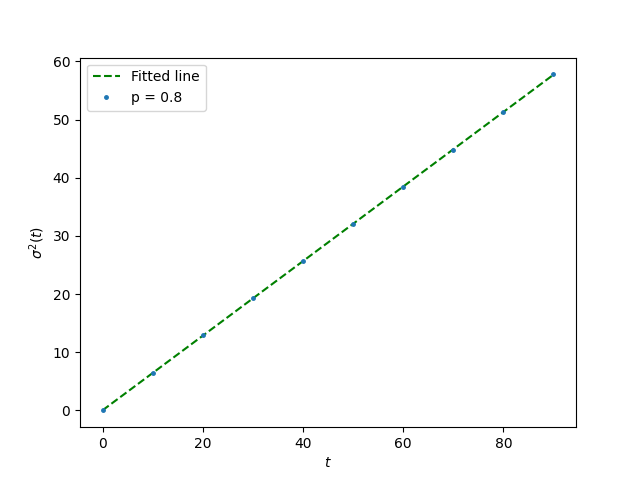
\includegraphics[width=\textwidth]{q2_var_0.8_100_10_100000.png}
    \caption{تغییرات واریانس مکان بر حسب زمان برای $p = 0.8$، $l = 1$، $\tau = 1$ و با $100\,000$ بار تکرار}
    \label{fig:q2_0.8_var}
  \end{minipage}
\end{figure}


\section{\textbf{ول‌گشت با تله}}
کد این بخش از تمرین را در فایل
\lr{q3.py}
می‌توان مشاهده نمود.
در ابتدا باید یک
\lr{object}
از کلاس
\lr{RandomWalkWith AbsorbingBarrier}
با طول دلخواه بسازیم.
سپس تابع
\lr{render}
را با مکان اولیه‌ی دل‌خواه صدا می‌زنیم.
روش کار این تابع به این صورت است که از بین اعداد
$1$
و
$-1$
به طور تصادفی و با احتمال برابر عدد انتخاب می‌کند و با مکان اولیه جمع می‌کند
تا زمانی که ول‌گشت به مرز‌ها برسد.
سپس زمان به دست آمده را به عنوان طول عمر ول‌گشت ذخیره می‌کند.
برای این که به طور آماری میانگین این مقدار را به دست بیاوریم، باید تابع
\lr{calc\_mean\_life\_time}
را با طول، گام و تعداد نمونه‌های مورد نظر فراخوانی کنیم.
این تابع داده‌های به دست آمده را در یک متغیر ذخیره می‌کند و سپس آن را برای استفاده‌های بعدی،
در یک فایل با فرمت
\lr{.npy}
می‌نویسد.
منحنی به دست آمده برای میانگین طول عمر ول‌گشت بر حسب مکان اولیه را در شکل‌
\ref{fig:q3_life_time}
می‌توان مشاهده نمود.
سهمی فیت شده به این نمودار از رابطه‌ی
\eqref{eqn:q3_fit_eqn}
پیروی می‌کند.
\\
اجرای این کد برای
$100\,000$
تکرار،
$137$
ثانیه زمان برد.

\begin{equation}
  \braket{\text{\lr{life time}}} = x_0 (18.98 - x_0) + 0.26
  \label{eqn:q3_fit_eqn}
\end{equation}

\begin{figure}[h]
  \centering
  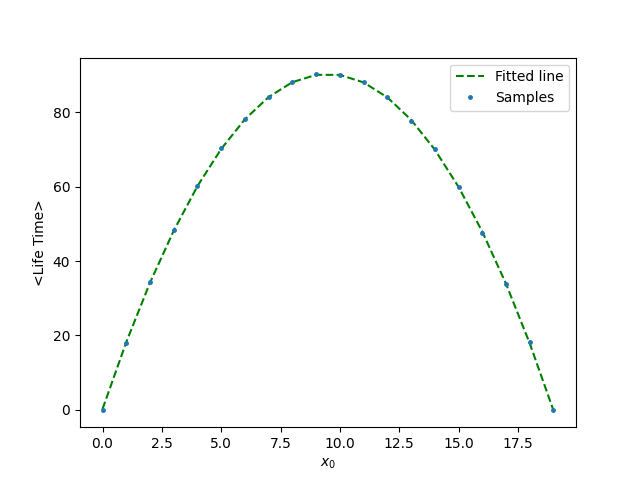
\includegraphics[width=.7\textwidth]{q3_life_time_20_1_100000.png}
  \caption{میانگین طول عمر ول‌گشت بر حسب مکان اولیه برای شبکه‌ای به طول $19$ و با $100\,000$ بار تکرار}
  \label{fig:q3_life_time}
\end{figure}


\section{\textbf{ول‌گشت با تله (الگوریتم تعینی)}}
کد این بخش از تمرین را در فایل
\lr{q4.py}
می توان مشاهده نمود.
ابتدا باید یک
\lr{object}
از کلاس
\lr{RandomWalkWith AbsorbingBarrier}
بسازیم.
سپس تابع
\lr{render}
را با مکان اولیه‌ی دل‌خواه صدا می‌زنیم.
روش کار این تابع به این صورت است که ابتدا یک لیست از احتمال حضور ول‌گشت در هر خانه می‌سازد.
سپس در هر مرحله احتمال هر خانه را نصف کرده و به دو خانه‌ی کناری خود در یک لیست جدید اضافه می‌کند.
مقدار احتمال‌هایی که در هر مرحله به مرز‌ها داده می‌شود، احتمال مرگ ول‌گشت در آن زمان است.
پس زمان را در این مقدار ضرب کرده و به میانگین عمر ول‌گشت اضافه می‌کنیم.
این کار را تا جایی انجام می‌دهیم که مجموع احتمال‌های مرگ، تا حد ممکن به
$1$
نزدیک شود.
برای به دست آوردن تغییرات متوسط طول عمر بر حسب مکان اولیه،
تابع
\lr{calc\_mean\_life\_time}
را با طول و گام مورد نظر فراخوانی کنیم.
این تابع داده‌های به دست آمده را در یک متغیر ذخیره می‌کند و سپس آن را برای استفاده‌های بعدی،
در یک فایل با فرمت
\lr{.npy}
می‌نویسد.
منحنی به دست آمده برای میانگین طول عمر ول‌گشت بر حسب مکان اولیه را در شکل‌
\ref{fig:q4_life_time}
می‌توان مشاهده نمود.
سهمی فیت شده به این نمودار از رابطه‌ی
\eqref{eqn:q4_fit_eqn}
پیروی می‌کند.
\\
اجرای این کد
$0.55$
ثانیه زمان برد.

\begin{equation}
  \braket{\text{\lr{life time}}} = x_0 (19 - x_0)
  \label{eqn:q4_fit_eqn}
\end{equation}

\begin{figure}[h]
  \centering
  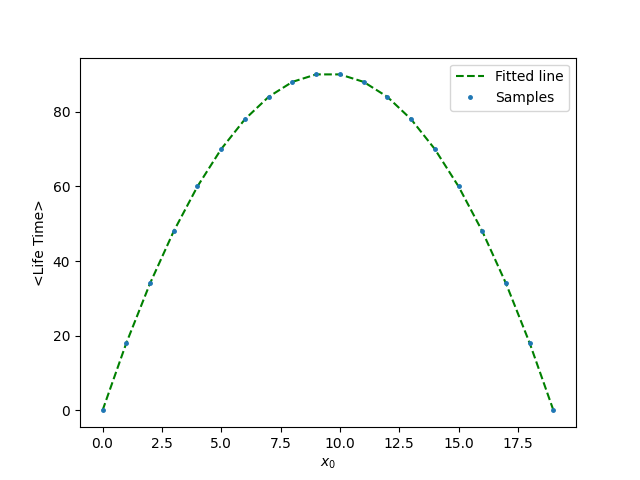
\includegraphics[width=.7\textwidth]{q4_life_time_20_1_.png}
  \caption{میانگین طول عمر ول‌گشت بر حسب مکان اولیه برای شبکه‌ای به طول $19$ با الگوریتم تعینی}
  \label{fig:q4_life_time}
\end{figure}


\section{\textbf{ول‌گشت دو بعدی}}
کد این بخش از تمرین در فایل
\lr{q5.py}
قابل مشاهده است.
کد این بخش کاملا مشابه با کد تمرین ۲ است،
تنها با این تفاوت که مکان‌ها به صورت یک عدد مختلط ذخیره می‌شوند
و در هر مرحله ول‌گشت به چهار جهت می‌تواند حرکت کند.
نمودار‌های به دست آمده برای طول گام‌های
$0.5$،
$1$
و
$2$
را در شکل‌های
\ref{fig:q5_0.5}
تا
\ref{fig:q5_2}
می‌توان مشاهده نمود.
شیب خطوط فیت شده به این نقاط نیز در جدول
\ref{tab:q5_slopes}
آورده شده است.

\begin{table}[h!]
  \centering
  \begin{tabular}{|c|c|c|c|}
    \hline
    $2$ & $1$ & $0.5$ & $l$ \\ \hline
    $3.997$ & $1.000$ & $0.250$ & $\frac{l^2}{\tau}$ \\ \hline
  \end{tabular}
  \caption{شیب خطوط فیت شده به نمودار‌ واریانس مکان ول‌گشت}
  \label{tab:q5_slopes}
\end{table}

همان‌طور که دیده می‌شود نتایج به دست آمده، مطابق با پیش‌بینی ما از تئوری هستند.

\begin{figure}[h!]
	\centering
  \begin{minipage}[b]{0.47\textwidth}
    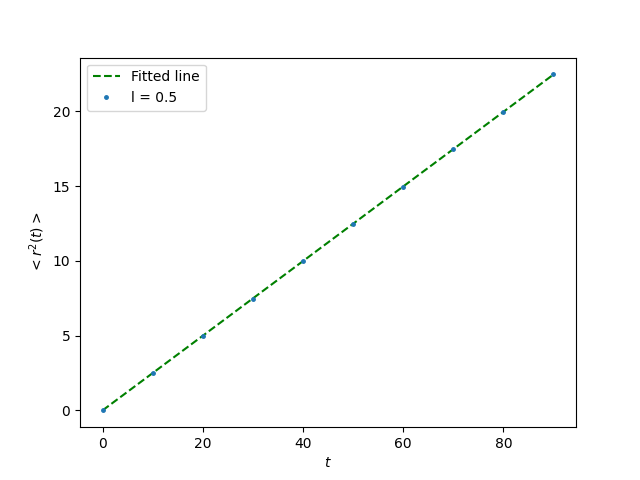
\includegraphics[width=\textwidth]{q5_var_0.5_100_10_100000.png}
    \caption{تغییرات واریانس مکان بر حسب زمان برای $p = 0.25$، $l = 0.5$، $\tau = 1$ و با $100\,000$ بار تکرار}
    \label{fig:q5_0.5}
  \end{minipage}
  \hfill
  \begin{minipage}[b]{0.47\textwidth}
    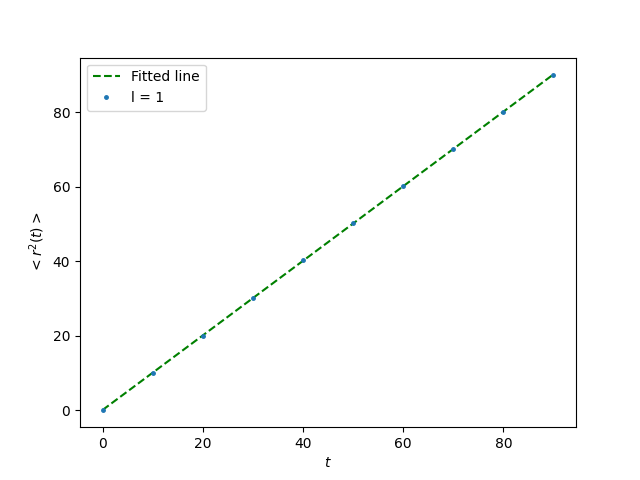
\includegraphics[width=\textwidth]{q5_var_1_100_10_100000.png}
    \caption{تغییرات واریانس مکان بر حسب زمان برای $p = 0.25$، $l = 1$، $\tau = 1$ و با $100\,000$ بار تکرار}
    \label{fig:q5_1}
  \end{minipage}
  \begin{minipage}[b]{0.47\textwidth}
    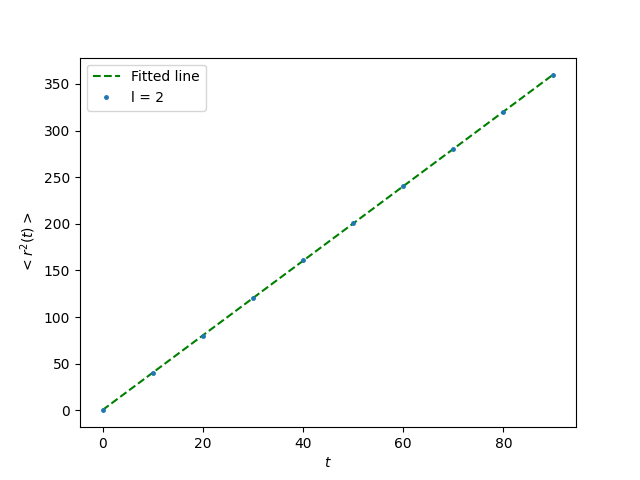
\includegraphics[width=\textwidth]{q5_var_2_100_10_100000.png}
    \caption{تغییرات واریانس مکان بر حسب زمان برای $p = 0.25$، $l = 2$، $\tau = 1$ و با $100\,000$ بار تکرار}
    \label{fig:q5_2}
  \end{minipage}
\end{figure}


\section{\textbf{\lr{Diffusion limited Aggregation}}}
کد این بخش از تمرین در فایل
\lr{q6.py}
قابل مشاهده است.
ابتدا باید یک
\lr{object}
از کلاس
\lr{DiffusionLimited Aggregation}
با طول دل‌خواه بسازیم.
سپس تابع
\lr{render}
را با زمان دل‌خواه صدا می‌زنیم.
شیوه کار این تابع به این صورت است که به طور تصادفی مکان اولیه‌ای برای ول‌گشت
در حداقل ارتفاع ممکن نسبت به خوشه پیدا می‌کند.
سپس مختصات به دست آمده را به تابع
\lr{\_\_final\_position}
پاس می‌دهد.
این تابع یک ول‌گشت را از آن نقطه شروع به حرکت می دهد تا نهایت یا از حد بالایی خارج شود و یا به خوشه بچسبد.
اگر از حد بالا خارج شده باشد مقدار
\lr{None}
و اگر چسبیده باشد مختصات نهایی را بر می‌گرداند.
تابع
\lr{render}
این حلقه را به قدری تکرار می‌کند تا به اندازه‌ی زمان داده شده، دانه به بذر اولیه چسبیده باشد.
برای نمایش خوشه‌ی به دست آمده، تابع
\lr{show}
را باید صدا بزنیم.
نتیجه‌ی نهایی را در شکل‌
\ref{fig:q6_diffusion}
می‌توان مشاهده نمود.

\begin{figure}[h!]
  \centering
  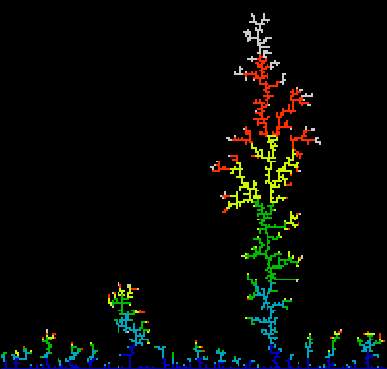
\includegraphics[width=.6\textwidth]{q6_200_2000.png}
  \caption{خوشه‌ی تجمع پخش محدود برای بذر خطی با طول$200$ و $2\,000$ ذره}
  \label{fig:q6_diffusion}
\end{figure}


\section{\textbf{ول‌گشت خودپرهیز}}
کد این بخش از تمرین در فایل
\lr{q7.py}
قابل مشاهده است.
برای رسم نمودار‌های خواسته شده باید تابع
\lr{show}
را با طول دلخواه صدا بزنیم.
روش کار این تابع به این صورت است که ابتدا تابع
\lr{count\_self\_avoiding\_paths}
را با طول داده شده صدا می‌زند.
این تابع در هر مرحله تعداد مسیر‌های بسته را می‌شمارد.
از آن‌جایی که هر مسیر‌ بسته برای طول
$l$،
$4^{(l^{'} - l)}$
مسیر بسته برای طول
$l^{'}$
خواهد بود، پس این تعداد به دست آمده را طبق قاعده‌ی بالا به تمام طول‌های بزرگ‌تر مساوی
$l$
اضافه می‌کنیم.
در نهایت داده‌های به دست آمده را در یک متغیر ذخیره کرده و برای استفاده‌های بعدی در فایلی با فرمت
\lr{.npy}
می‌نویسیم.
نمودار‌های خواسته شده را در شکل‌های
\ref{fig:q7_count}
و
\ref{fig:q7_percentage}
می‌توان مشاهده نمود.
همان‌طور که مشاهده می‌شود،
نسبت تعداد گشت‌های خود‌پرهیز به تعداد کل گشت‌ها با افزایش
$N$
به صفر میل می‌کند که مطابق با انتظار ما است.
داده‌های به دست آمده، در جدول
\ref{tab:q7_self_avoid_paths}
آورده شده است.

\begin{table}[h!]
  \centering
  \begin{tabular}{|c|c|c|c|c|c|}
    \hline
    گشت‌های خودپرهیز & $N$ & گشت‌های خودپرهیز & $N$ & گشت‌های خودپرهیز & $N$ \\ \hline
    $881500$ & $13$ & $2172$ & $7$ & $4$ & $1$ \\ \hline
    $2374444$ & $14$ & $5916$ & $8$ & $12$ & $2$ \\ \hline
    $6416596$ & $15$ & $16268$ & $9$ & $36$ & $3$ \\ \hline
    $17245332$ & $16$ & $44100$ & $10$ & $100$ & $4$ \\ \hline
    $46466676$ & $17$ & $120292$ & $11$ & $284$ & $5$ \\ \hline
    $124658732$ & $18$ & $324932$ & $12$ & $780$ & $6$ \\ \hline
  \end{tabular}
  \caption{تعداد گشت‌های خود‌پرهیز بر حسب $N$}
  \label{tab:q7_self_avoid_paths}
\end{table}

\begin{figure}[h!]
	\centering
  \begin{minipage}[b]{0.48\textwidth}
    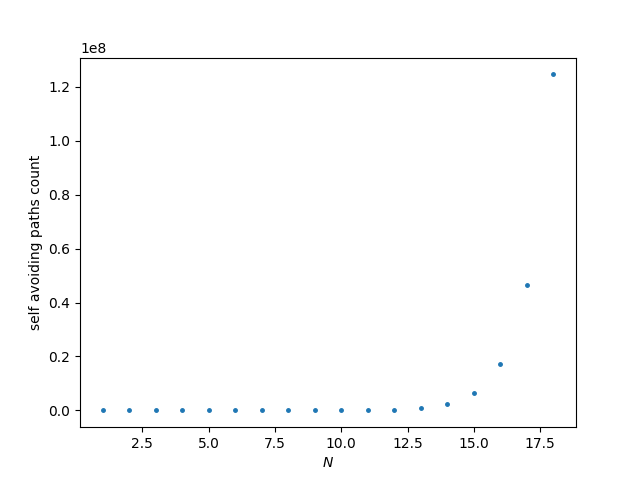
\includegraphics[width=\textwidth]{q7_self_avoiding_count_18.png}
    \caption{تعداد گشت‌های خود‌پرهیز ممکن بر حسب $N$}
    \label{fig:q7_count}
  \end{minipage}
  \hfill
  \begin{minipage}[b]{0.48\textwidth}
    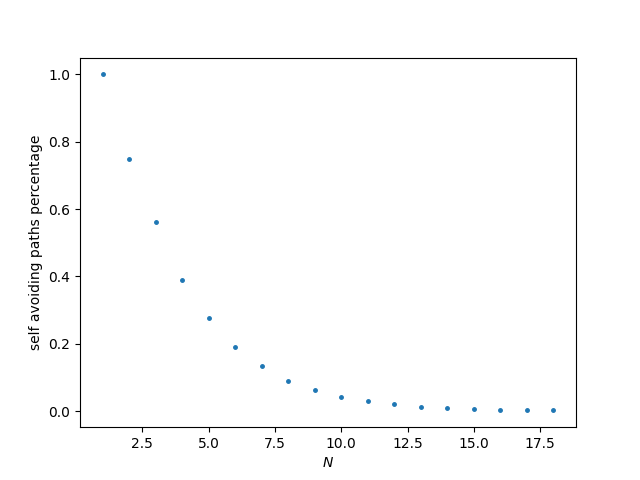
\includegraphics[width=\textwidth]{q7_self_avoiding_percentage_18.png}
    \caption{نسبت تعداد گشت‌های خود‌پرهیز بر تعداد گشت‌های آزاد بر حسب $N$}
    \label{fig:q7_percentage}
  \end{minipage}
\end{figure}

\end{document}
